% TODO: make all requirements navigateable (press on one and it scrolls the document to the bottom). 
% TODO: can 

% =============================================================================
% =============================================================================
% HEADER										
% =============================================================================
% =============================================================================

\documentclass[11pt]{article}
\author{Sami Farhat}
\title{STE}

% -----------------------------------------------------------------------------
% Packages

\usepackage{titlesec} 				% to change the section font-size
\usepackage[margin=0.8in]{geometry} % for Margins
\usepackage{geometry}
\usepackage{hyperref}				% for links
\usepackage{multicol}				% for embedding lists in multiple-columns
\usepackage{enumitem}				% customize lists
\usepackage{fontspec}				% customise font used
\usepackage{tabularx}
\usepackage{soul}
\usepackage{color} 					% colouring text
\usepackage{array}					% bold table column
\usepackage{booktabs}				% http://ctan.org/pkg/booktabs
\usepackage{etoolbox}
\usepackage{float}
\usepackage[table]{colortbl}		% http://ctan.org/pkg/xcolor
\usepackage{tikz}					% for hierarchy structure
\usepackage[export]{adjustbox}
\usepackage{wrapfig}
\usepackage{graphicx}
% Code - use minted instead of listings
% \usepackage{listings}
\usepackage{minted}					% better than listings for code highlight
\usepackage{tocloft}				% customize Table of Contents
\usepackage{fancyhdr}				% for page numbering
\usepackage{lastpage}				% for page numbering
\usepackage[autostyle, english = american]{csquotes} % makes quotes sane 
\usepackage[super]{nth}             % formats 1st, 2nd, 3rd automatically 

% General 
% -----------------------
\MakeOuterQuote{"} % to make double quotes work

% Font
% -----------------------
% \setmainfont{Helvetica}

% Items
% -----------------------

\setlist[itemize]{leftmargin=15pt}
\def \tableitemsep {0pt}
\def \tableleftsep {10pt}

% Graphics
% ---------------------
\graphicspath{ {res/} }

% Page numbers 
% ------------------------
\pagestyle{fancy}
\fancyhf{}
\rfoot{Page \thepage \hspace{1pt} of \pageref{LastPage}}

% Sections
% ---------------------
\setcounter{section}{0}
% TODO: make sections have a pagebreak before them
% no numbering of sections 
% \setcounter{secnumdepth}{0}

% Tables
% ---------------------
% increase margins of tables (1 is default)
\def\arraystretch{1.5}

\newcommand{\tblitembegin} {
\vspace{-\topsep}
\begin{itemize}[noitemsep, topsep=0pt,itemsep=-1ex,partopsep=1ex, parsep=1ex,leftmargin=*,]
}
\newcommand{\tblitemend} {
\end{itemize}
\vspace{-\topsep}
}
% for line breaks in table
\newcolumntype{b}{X}
\newcolumntype{s}{>{\hsize=.5\hsize}l}

\newcommand{\specialcell}[2][l]{%
\begin{tabular}[#1]{@{}l@{}}#2\end{tabular}}

\newcommand{\tblheader}{\textbf}
\definecolor{listinggray}{gray}{0.9}
\definecolor{lbcolor}{rgb}{0.9,0.9,0.9}

% Paragraphs
% --------
% remove paragraph indent
\setlength{\parindent}{0pt} 
\parskip=10pt

% Table of Contents 
% -----------------------------------
% \cftsetindents{section}{0em}{2em}
% \cftsetindents{subsection}{0em}{2em}
% \renewcommand\cfttoctitlefont{\hfill\Large\bfseries}
% \renewcommand\cftaftertoctitle{\hfill\mbox{}}

% References 
% ----------
\newcommand{\ROne}{\hyperref[req:r1]{R1}}
\newcommand{\RTwo}{\hyperref[req:r2]{R2}}
\newcommand{\RThree}{\hyperref[req:r3]{R3}}
\newcommand{\RFour}{\hyperref[req:r4]{R4}}
\newcommand{\RFive}{\hyperref[req:r5]{R5}}
\newcommand{\RSix}{\hyperref[req:r6]{R6}}
\newcommand{\RSeven}{\hyperref[req:r7]{R7}}
\newcommand{\REight}{\hyperref[req:r8]{R8}}

% Code 
% ----
\newmintinline{java}{}
\newminted{java}{
frame=single, 
showtabs=false, 
showspaces=false
}
% \lstset{
% language=Java,
% upquote=true, 
% breaklines=true,  % sets automatic line breaking
% %breakatwhitespace=false, % sets if automatic breaks should only happen at whitespace
% showspaces=false,
% showstringspaces=false,
% % basicstyle=\ttfamily, % change this for different font-sizes
% basicstyle=\small,
% %numbers=left,
% %numberstyle=\tiny,
% frame=single,
% %commentstyle=\color{gray}
% keywordstyle=\color[rgb]{0,0,1},
% commentstyle=\color[rgb]{0.133,0.545,0.133},
% stringstyle=\color[rgb]{0.627,0.126,0.941}
% }

% =============================================================================
% =============================================================================
%  CONTENT									
% =============================================================================
% =============================================================================

\begin{document}

% ============================================================================ 
% TITLE PAGE
% ============================================================================ 

\clearpage
%\maketitle
\thispagestyle{empty} % remove page number
\pagebreak 
\begin{titlepage}
\begin{center}
\vspace*{1cm}
{\Huge Software Testing} \\
\vspace{0.5cm}
{\LARGE STE\\}
\vspace{0.5cm}
\vspace{3.5cm}
{\LARGE Sami Farhat\\}
\vspace{0.1cm}
{\Large \# 1065452\\}
\vspace{0.3cm}
\vfill
\vspace{0.8cm}
Software Engineering Programme\\        
Computer Science\\
\vspace{0.5cm}
University of Oxford\\
United Kingdom\\
\vspace{1.0cm}         


\includegraphics[width=0.15\textwidth]{oxford-logo.png}
\end{center}
\end{titlepage}

% ============================================================================ 
% TABLE OF CONTENTS
% ============================================================================ 

\clearpage
\tableofcontents 
\thispagestyle{empty} % remove page number
\pagebreak
\pagenumbering{arabic} % start numbering  

% ============================================================================ 
% FIGURES & TABLES
% ============================================================================ 

\thispagestyle{empty}
\listoffigures
\listoftables 

% ============================================================================
% REQUIREMENTS 
% Requests for improvements on the requirements. 
% TODO: would be great if we could write the requirements as we understood them.
% TODO: Talk about our impression from reading the system requirements and all the vaguenesses found in there. 
% ------------------------------------------------------------------------------------------------------------
\section{System Requirements}

This section presents a review of the set system requirements, identifying those that are considered ‘unclear’, vague, or requirements that may be classified as defects in the specifications.  Once identified, assumptions will be made to manage such requirements.
\par
The source or basis of such system specifications has not been made identified during the course of this work.  Hence, should a more comprehensive reference document be made available, such as IEEE SRS, which can be reviewed, then development would be greatly simplified, and the output would present a clearer guide, with fewer ambiguities. Testing of specification and the basis on which these were selected are critical to the work, particularly in the test phase. Test trials based on false, incomplete, or unclear specifications, may generate many false-positive or even worse false-negatives and may prove costly both in terms of development time and development cost.

% In this section we shall review the provided requirements calling attention to mistakes and vaguenesses in the requirements, which we recognise as defects. As well as identifying them, we shall delineate any assumptions we are forced to make due to missing or imprecise requirements. 
% % Type of Req Document? Informal? 
% % -------------------------------
% It is not evident at the outset the type of specification document these requirements were extracted from; if a more complete document is available, such as an IEEE SRS, then we would kindly request access to it as it should help in filling the voids left by the current extact.  
% This step is critical before proceeding with the test process as testing based on false or incomplete understanding risks generating lots of false-positive or worse false-negatives, and would be costly both in terms of time and money. 
% \par

% -------------------------------------------------
% Requirements organisation (bullets, no numbering)
% -------------------------------------------------
\subsection{Organisation of Requirements}
Requirements are presented in the form of bullets, whereas a numbering scheme would have provided a smoother workflow, since those testing or reviewing the test document would reference individual requirements using specific identifiers.  In some organisations, test methods or test classes are prefixed with the requirement reference being addressed.
\par
A part of the work involved labelling requirements for the workflow process presented in the form of a table, as shown in Appendix \ref{app:labelled-requirements}.  Therefore as good practice, it is recommended that additions or alterations to be made to requirements are actually amended on the reference table.

% The requirements are bulletised, a numbering scheme would be much more apt as it allows testers and reviewers of the document the ability to reference individual requirements using their identifier. In some organisation, test methods or classes are prefixed with the requirement reference they address. 
% We will take it on ourselves to label the requirements for our own workflow (see appendix \ref{app:labelled-requirements}) and we propose that any additions or alterations to be made on the requirements be done on that table.

% TODO: Some SRS documents will capitalise SHOULD, MUST, MAY to leave no room for confusion. 

% --------------------------------------------------
% Requirements doc lacks of coherence 
% which lends to an overall lack of professionalism
% --------------------------------------------------
\subsection{Coherence of Requirements}

At a first glance, it becomes apparent that there is a lack of coherence in the structure and wording of requirements, which indicates a lack of a formal and systematic approach in the software engineering process.  A positive spin-off of this surprisingly may be that it alerts the tester on what he is to expect in the quality of software under test, hence may question project management procedures in place, and as a result the Developer’s approach and end-result.
\par
Below some of the non-coherences observed are listed. These are by no means critical, but may be flagged as defects.
\begin{itemize}
    \item The first bullet in the list (\textit{"The PTMA must implement a Personal Tax Management System to meet the following requirements."}) is not an explicit requirement, but an introductory sentence which would better be presented without a bullet and is misleading to the reader. 
    \item The seventh bullet in the list (\textit{"The system must include a simple ‘help’ system that lists all commands"}) does not terminate with a full stop while the rest do. 
    \item Requirements (\REightFive \space to \REightTen) all commence with \textit{Calculation of tax for people}, whereas the last two requirements (\REightEleven \space to \REightTwelve) commence with \textit{Calculation for people}. It is not evident why different wording was opted for between these requirements. 
    \item The bullet detailing the taxing of divorced people (\REightSeven) does not capitalise the word "divorced", but does capitalise "Single" and "Married". Readers should attempt their not to take this as a lack of respect for divorced individuals. 
%   % in the When outlining marital status taxing, we can see "Calculation of tax for Married people", "Calculation of tax for Single people", but the word 'divorced' is not capitalised, typo or lack of respect for divorced?  
\end{itemize}


% ----------------------------------------------
% Non-Functional Requirements
% ----------------------------------------------
\subsection{Non-functional Requirements}
\label{sec:non-functional-requirements}
It is understood that performance testing, security, and other non-functional requirements are not within the scope of testing for this project.
However, including such items in the system requirements review is essential as they constitute an integral part of the requirements development process. It is usually expected that requirements on security, performance, compatibility and robustness are elicited clearly in a separate non-functional requirements section.  However, it may well be that the scope of testing is restricted to functional aspects.
\par
Despite this, the following is identified (\RSeven: \textit{"The system must not crash if the user enters something that they are not meant to."}) as a non-functional requirement pertaining to the robustness of the application. In a more formal document, this requirement would be separated from functional requirements.

% ----------------------------------------------
% Key term definitions
% ----------------------------------------------
\subsection{Key term definitions}
\label{sec:key-term-definitions}

Some key sections required in a typical SRS document are missing from the requirements.  As an example, a "Definitions" section outlining the meaning of key terms used in the requirements is missing.  It is also important to note that terms such as "will", "should", "must", or "may", must conform to a predefined standard definition (e.g. IEEE Std), in order to ascertain their priority over each other, hence avoiding confusion in the interpretation of each term. The importance of this is not to be under-estimated particularly that it is likely that the audience of the document will include non-native English speakers.
\par
Furthermore, the exact explicit definition of the below keywords is absolutely essential, in view of the fact that terms appear to be used interchangeably:
\begin{itemize}
    \item Client, Customer, and Person - Client is used in requirements (\ROne, \RTwo, \RFive), Customer is used in (\RTwo, \RThree, \RFour, \RFive), and Person is used in all (\REight) requirements. \RFive \space interchangeably uses Customer and Client within the same sentence. 
    \item System and Application - System is used in (\RTwo, \RSix, \RSeven), while Application is used in (\ROne, \RFour, \RFive). 
\end{itemize}
It is assumed through contextual understanding that these refer to the same entity.  However, confirmation and a more precise definition of the terms must be presented in a formal document.

% It is good that the present requirements limit the key terms used to a subset of well-known ones (will, may, should, must) are used. This reduces the risk of vagueness emanating from (english understanding). 

% --------------------------------------
% DEFECTS and VAGUENESS in requirements 
% --------------------------------------
\subsection{Defects and Vaguenesses}
\label{sec:defects-and-vaguenesses}
In this section we address imprecise or 'loose' requirements, which are believed to truly form defects in requirements.
These have been labelled (see appendix \ref{app:labelled-requirements}) to improve readability and accessibility of the report.

% [1] -----------------------------------------------------------------------------
\subsubsection{The application must enable the storage of client’s personal details including [R1]}
The term storage is not clear in that it does not specify where details are to be stored. 
Storage may be permanent (e.g. database, file on system...) or in-memory surviving only until the next launch or boot up. 
\par
If persistent storage is to be used, then more details on how thi storage should behave, its robustness, portability, responsiveness would be needed. 
\par
For testing purposes within this work, it is assumed that the storage of details need only be in-memory when the application is running, as such, no testing has been done on permanent-storage.

% [2] -----------------------------------------------------------------------------
\subsubsection{The software should issue each customer a numeric identifier [R2]}
This requirement was found to be clear and unambiguous. 
One minor comment is presented here, which is that usage of the word 'die' is not entirely appropriate, even if quoted. However, software does tend to use questionable wording (think of the POSIX function kill), so this may not be a major issue.  

% [3] -----------------------------------------------------------------------------
\subsubsection{The PTMA should enable customer details to be updated [R3]}
This requirement was found to be clear and unambiguous at first read. 
However, after noting that the implementation contains sizeable chunks of code pertaining to client updates (four menu commands each with its own method definition), testers would question whether there is a lack of specificity from the requirements perspective, or going over the requirements by the developers. 
\par
In both cases, it is not clear and is surprising why for example the 'salary' field cannot be updated with one command, as the case for 'first-name', 'last-name' and 'tax-code'.  
\par
Moreover, this requirement may be improved by specifying that customer IDs cannot be updated in order to avoid any possible confusion during implementation. 

% [4] -----------------------------------------------------------------------------
\subsubsection{The application should be able to print lists of customer information [R4]}
% with users being able to select blocks of customers to be printed based on their unique identifiers.}
This requirement is clear and unambiguous. 
By being less specific on how the user is expected to specify the blocks to print, the requirement provides developers with the flexibility, which is needed seeing as (\RFour) has strong dependency on the choice of identifiers used in (\RTwo). If non-integer identifiers were used in \RTwo \space then printing blocks of users may have to be done using comma-separated input from the user. 

% [5] -----------------------------------------------------------------------------
\subsubsection{The application will calculate the tax amount to be paid by each client [R5]} 
% and display this amount along with the other customer details. The amount of the tax is based on their taxcode and their current salary according to the rules below.}
This requirement is clear and unambiguous. 
However, it remains unclear why it is separated from the tax rules (R8.x), reason may well be that these could have been structured to follow each other. 

% [6] -----------------------------------------------------------------------------
\subsubsection{The system must include a simple 'help' system that lists all commands [R6]}

This requirement was found to be clear and unambiguous, assuming 'system' and 'application' refer to the same thing (see section \ref{sec:key-term-definitions}). 

% [7] -----------------------------------------------------------------------------
\subsubsection{The system must not crash if the user enters something that they are not meant to [R7]}
Assuming 'system' refers to the application, the requirement is clear. 
This requirement relates to the application's robustness and should in a more formal document  be placed in the non-functional requirements section along with other requirements relating to performance, robustness, security (see section \ref{sec:non-functional-requirements}).

% [8] -----------------------------------------------------------------------------
\subsubsection{Tax Rules [R8]}

In this sub-section comments on defects found in requirements (R8.x) are provided, without necessarily delving into each requirement as many of these share the same defects.

% ----------------------------------
% Mutual exclusivity of tax brackets 
% ----------------------------------
\paragraph{Mutual exclusivity of tax brackets:}
Requirement (\REightFour) does not specify the existence of any mutual exclusivity between tax letters in the same tax groups i.e. between: 
\begin{itemize}[noitemsep]
\item 'M', 'S', and 'D' 
\item 'C', 'E', and 'F'
\item 'T' and 'U'
\end{itemize}
This will be assumed since logically a person cannot simultaneously have both (2 children) and (1 child), therefore cannot be in both groups. Similarly, one's marital status cannot be both single and divorced, hence the mutual exclusivity.  

% --------------------------------------
% Marital Status is required in tax code
% --------------------------------------
\paragraph{Marital status is required in tax code:}
Requirement (\REightFour) does not specify that the tax code MUST contain a marital status. There are many reasons why this can be justifiably assumed to be a missing requirement: 
\begin{enumerate}
	\item Requirements (\REightEight) and onwards all indicate that the tax to be calculated for their respective brackets has to be done after the Marital status tax has been applied. This suggests that some tax due to Marital status must have previously been applied. 
	\item Should it be possible that Marital status be absent from the tax code, then it would become possible for a tax code not to have any letters at all. This would conflict with requirement (\REightTwo). % This can happen if they have no Marital status, no children and are not in education. 
	% \item The reader is not aware of a marital status that does not belong outside of married, divroced, single. Common sense employed here. 
\end{enumerate}

% -----------------
% Unusual tax rates
% -----------------
\paragraph{Unusual tax rates \& negative salaries:}
The unusual tax rates were brought to the attention of the reader in the assignment notes, hence there is no call for pointing them out as a defect. However, in view of the possibility of a tax payer earning a salary and paying all of it and more to the government (when tax rate > 100\%), one must ask whether negative salaries as a concept exist in Failovia. 
\par
It is not clear from the requirements how the application should respond to a user-provided negative salary or base amount. As testers, we would expect two valid application responses to negative salaries: 

\begin{enumerate}
	\item Calculate the tax from the negative salary leading to a negative tax. In practical terms, this means the tax authorities owe the client some money.
	\item Provide a user error when a negative salary of negative tax amount is input. 
\end{enumerate}

It is preferable that the approach that the application must undertake should be presented clearly in the requirements.

% --------------------------
% Contradictory requirements
% --------------------------
\paragraph{Contradictory requirements:}
The below requirement (\REightFive) is not correctly worded and may be interpreted differently by developers, whom it is believed may well have implemented the code based on what one would have expected the requirement to mean, rather than what it actually elicited. 
\par
\begin{figure}[H]
\begin{mdframed}
{
\it
\footnotesize
Calculation of tax for Married people: one of the following four bands will apply:
\begin{itemize}
	\item Married people with a current salary of less than £5000 will pay a tax rate of
	70\% of their base tax amount.
	\item Married people with a current salary less than £12,000 will pay a tax rate of
	90\% of their base tax amount.
	\item Married people with a current salary less than £27,000 will pay a tax rate of
	120\% of their base tax amount
	\item Married people with a current salary above than £27,000 will pay a tax rate
	of 130\% of their base tax amount
\end{itemize}	
}
\end{mdframed}
\caption{Requirement \REightFive}
\end{figure} 


It is noted from the above that the bullets contradict the ones preceding them: for someone earning £3,000 in salary, the first bullet implies they should pay a tax rate of 70\%, the second overrides the first bullet and implies they should pay 90\%, the third one 120\% and the fourth one 130\%. It is believed that the intention behind the bullets is to establish tax brackets as below: 
\begin{itemize}
	\item People earning £0 - £5,000 should pay 70\% tax rate 
	\item People earning £5,000 - £12,000 should pay 90\%
	\item People earning £12,000 - £27,000 should pay 120\%
	\item People earning over £27,000 should pay 130\%
\end{itemize}
The same applies for all subsequent requirements \REightSix \space to \REightTwelve. 

% Different tax rates for the same bracket
Requirements (\REightSix \space and \REightSeven) have contradictory third and fourth bullets which state different tax rates for the same tax brackets. Looking at the rest of the requirements we infer that this defect is due to a typo in the third bullet of \REightSix \space and \REightSeven. 

It is believed that the intention is as presented as below: 
\begin{itemize}
	\item People earning £11,000 - £22,000 should pay a rate of 125\%
	\item People earning £22,000 and above should pay a rate 132\%
\end{itemize}

% -------------
% EDGE SALARIES 
% -------------
\paragraph{Edge salaries:}
% 8 - Married section 
The requirements for taxing married people do not cover those who earn exactly £27,000. The third bullet ("less than") implies they are excluded from the 120\% tax rate, and the bullet right after ("above than") excludes them as well. 
\par
Salaries that are not covered by the requirements are summarised in the following:
\begin{itemize}
	\item Married and earning £27,000
	\item Single and earning £22,000
	\item Divorced and earning £24,000
	\item Single Child and earning £10,400
	\item Two children and earning £9,900
	\item More than 2 children and earning £9,000
	\item FT education below 24 and earning £3,000
	\item FT education 24 and above earning £3,000
\end{itemize}

% Would be helpful 
% [ Thus, for clarity, both of the following tax codes are valid. ] 
% It would be extra helpful to provide a tax code that should not be accepted (e.g. 1080MT90). In fairness the provided examples were appreciated as they helped clarify the requriement.
% --------------------------------------
% MISSING REQUIREMENTS ? 
% --------------------------------------
\subsection{Missing requirements}

% Delete clients. 
There are no requirements for the user's ability to delete customers from storage. This is tacitly mentioned as part of the second requirements relating to ID uniqueness. It is believed that it is then an oversight on the requirements' writers. 
\par
% Show ID of clients. 
Requirement (\RFour) points to the need for allowing users to see customers based on their IDs. However, there is no reference to how the application-generated IDs are presented to the user. This was found to be an issue during exploratory testing, and was sourced back to both a defect in the implementation and absence in the requirements. 
\par
% Edge case: Negative salaries. 
The question arises, is it implicit that negative salaries are not a thing, and how could the code deal with that? 
\par
% Edge case: taxcode with duplicate tax letters
The requirement does not specify the application's behaviour for the case when duplicates of the same letter are found in the tax code. We would expect the tax code parser to complain and specify this as invalid, however others may interpret "DD1000" to be apply the Divorced taxing twice. 

% --------------------------------------
% Assumptions
% --------------------------------------

\subsection{Assumptions}
Requirements were reviewed and assumptions made in the testing are listed as in the following.
\begin{itemize}
    \item It is assumed that requirements do not require persistent storage of customer details.
    \item Tax letters in the same group are mutually exclusive. 
    \item Tax code MUST contain a Marital status letter. 
    \item Tax for Married people - It is assumed "above than or equal to £27,000" pay 130\%. 
    \item Tax for Single people - It is assumed that "less than £22,000" pay 125\%. 
    \item Tax for Single people - It is assumed that "above than or equal £22,000" pay 132\%. 
    \item Tax for Divorced people - It is assumed that "less than £24,000" pay 95\%.
    \item Tax for Divorced people - It is assumed that "above than or equal £24,000" pay 110\%.
    \item It is assumed that that negative salaries and base amounts are invalid.
    \item It is assumed that lower case tax-letters are NOT equivalent to their respective upper-case letter. 
\end{itemize}
% \subsection{Assumptions}
Requirements were reviewed and assumptions made in the testing are listed as in the following.
\begin{itemize}
    \item It is assumed that requirements do not require persistent storage of customer details.
    \item Tax letters in the same group are mutually exclusive. 
    \item Tax code MUST contain a Marital status letter. 
    \item Tax for Married people - It is assumed "above than or equal to £27,000" pay 130\%. 
    \item Tax for Single people - It is assumed that "less than £22,000" pay 125\%. 
    \item Tax for Single people - It is assumed that "above than or equal £22,000" pay 132\%. 
    \item Tax for Divorced people - It is assumed that "less than £24,000" pay 95\%.
    \item Tax for Divorced people - It is assumed that "above than or equal £24,000" pay 110\%.
    \item It is assumed that that negative salaries and base amounts are invalid.
    \item It is assumed that lower case tax-letters are NOT equivalent to their respective upper-case letter. 
\end{itemize}

% --------------------------------------
% END OF REQUIREMENTS
% --------------------------------------
% ============================================================================

% ============================================================================
% CODE READ
\pagebreak
\section{Code Review}
% Detail what notes were taken when reading the code and what was noticed from afar
% We should say that reading the code is not great in that it usually focuses our testing on some things and push us not to test, things that 
% we expect to be correct (given we know the implementation). As such, it is always better to try and make no assumptions about the contents 
% of the code when writing the tests. 
% =========================================================================
\section{Code Review}

% =========================================================================
% Code structure 
% =========================================================================
% 1 - Assess the structure of the code.

\subsection{Code Structure} 
\label{sec:code-structure}
Overall, the code is difficult to read in partly due to the lack of coherence and consistency with the coding style and the lack of useful documentation, but mostly due to questionable implementation choices. 

Below, we shall focus on the code's structure and testability. Critique of the code that is unrelated to its testability can be found in Appendix \ref{app:code-critique}. 

\begin{itemize}
	\item We note that error reporting in the application is weak: no exceptions thrown anywhere, none of the implemented methods return booleans or integers that could report errors (like returning -1 to indicate an error). There are no means by which  to valid errors occurrences in methods, such as when the ID provided in the delete method is not owned by any customer. 
	\item There are many instances of duplicated code that should have been separated in a private method to be called by others (deleteCustomer, updateCustomer) all attempt to find a customer with the given ID. 
\end{itemize}

% =========================================================================
% Code testability & Recommendations  
% =========================================================================
% 2 - Comment on its testability 

\subsection{Code testability \& Recommendations}
The items below are identified as hindrances to the testing work.  Each item is described and suggestions to improve the structure are provided.

% ----------------------------------------------------------------------------
\subsubsection{Error reporting}
\label{sec:error-reporting}
The application provided exhibits weak and badly structured error reporting. We would normally expect methods in underlying classes to throw exceptions on invalid inputs and report their results to methods higher up the stack via booleans or return objects. These high level methods would then evaluate the return-code or try/catch exceptions thereby generating a readable user output where appropriate.
\par
Such a design would allow reliable testing capabilities of underlying methods while also protecting the user from confusing and verbose error messages. 
\par 
Part of the refactoring carried out involved throwing exceptions upon certain error conditions so that the test framework could catch those exceptions and evaluate the reasons for their throwing. 
This is especially relevant to testing \javainline{TaxEngine} whose input tax code may be invalid, in which case we would hope and expect an exception to be thrown. 
\par 
We create \javainline{TaxCalcException} as a child of RuntimeException; the reason for it inheriting from RuntimeException and not Exception is that it allows us to avoid needing to add snippets \javainline{throws TaxCalcException} after every method definition hence polluting the code base. 
This approach was deemed less intrusive. 
% ----------------------------------------------------------------------------

% ----------------------------------------------------------------------------
\subsubsection{Static Main}

By design, the application's Main class is primarily static, meaning that there are only one Scanner and AllCustomers objects during the process' runtime. This is problematic in that it allows state to be maintained across different test runs leading to more tightly coupled feature scenarios.
\par
A solution to this is to remove static modifiers from the Main class forcing developers and testers to instantiate their own objects. This provides a much neater approach, one that is much less likely to lead to errors in testing. 
\par
Additionally, some of our tests will look to dependency-inject our own test objects into Main to be used (sections \ref{sec:main-stdio}, \ref{sec:allcustomers-inject}). An overview of the changes made can be seen below.
\begin{itemize}
	\item remove static modifiers from the class's members and methods.  
	\item add a default constructor.
	\item update the \javainline{main} method to instantiate Main, via \javainline{Main main = new Main();}.
	\item switch to making method calls on the instance rather than static methods. 
\end{itemize}

% -----------------------------------------------
\begin{minipage}[b]{0.5\textwidth}
\begin{figure}[H]
\centering
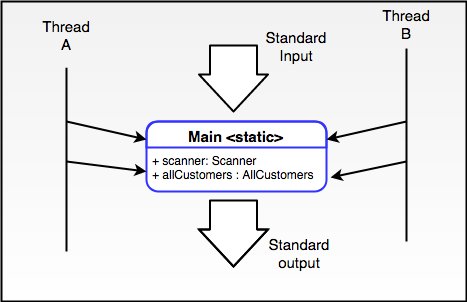
\includegraphics[scale=0.4]{res/STE-Page-1-original.png}
\caption{Before changes: one static Main}
\end{figure}
\end{minipage}
% -----------------------------------------------
\begin{minipage}[b]{0.5\textwidth}
\begin{figure}[H]
\centering
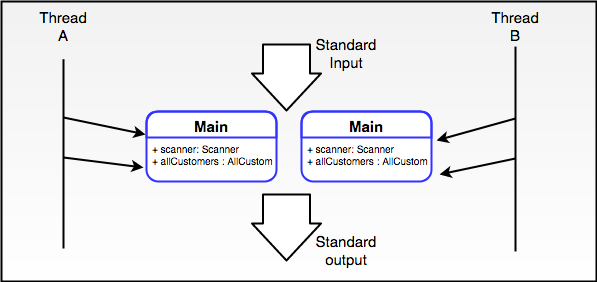
\includegraphics[scale=0.4]{res/STE-Page-2-original.png}	
\caption{After changes: different instances of Main}
\end{figure}
\end{minipage}
% ------------------------------------------------

The above steps improve encapsulation of state within Main instances and reduce the number of shared resources between threads but are not sufficient. There are still only one standard input and one standard output contended on by all threads. Below we describe how we get around this contention.

% -------------------------------------------------------
\subsubsection{Main: Standard I/O}
\label{sec:main-stdio}
The application, being command-line driven, relies on stdin for user input and stdout for output. Testing the software in a behaviour driven methodology necessitates injecting input to stdin to simulate user input and inspecting the output from stdout to verify correctness. 
\par
To validate the output of the application, the tester needs to redirect stdout to a stream from which the string can be extracted and inspected. A quick solution to this, and one that does not require any code changes on behalf of the application under test, is to call \javainline{System.setOut(printStream)} prior to the start of the tests; this effectively redirects all output which would have otherwise gone to stdout into the printStream; which can then be used by the tester for checking. 
\par
An issue with this approach is that System.in is shared by all components of the Java executable which in a test environment includes the test suite as well as all instances of the application being tested (Main in this case). Recall that test suites often run test methods in parallel; this can lead to multiple Main instances running simultaneously and appending output to the same stream. Even worse is that the Cucumber-JVM shares the same stdout and may choose to output its debug info or test results to it as well. 
\par 

\paragraph{Recommendation:}
In order to isolate the standard input and output of each Main instance and to facilitate testing, class members of type PrintStream and InputStream are introduced in Main class and would allow callers to Main's constructor to inject those streams.
\par
This allows us to provide specific streams for Main to work with when running the instance in a test environment where we would like to exert control and inspect the streams. 
\par 
Following our changes, creators of Main can either choose to provide their own streams or stick to the default stdin and stdout by calling Main's default constructor. 
\par
Another class in the application uses System.out to print and that is AllCustomers. It was debated whether we should dependency inject the streams to print to as well, but as there exists only one method concerned with printing in AllCustomers: `printCustomers`, it was decided that adding another \javainline{printCustomers} method taking in a PrintStream would suffice.
\begin{figure}[H]
	\centering
	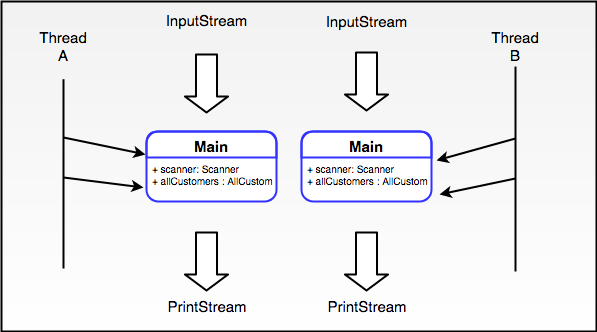
\includegraphics[scale=0.4]{res/STE-Page-3-original.png}
	\caption{After addition of PrintStream \& InputStream to Main class}
\end{figure}
% We would encourage considering a software redesign, limiting the span of objects that may write to stdout or read from stdin. [ Can expand on this more? ]
\par
% ----------------------------------------------------------------------------

% ----------------------------------------------------------------------------
\subsubsection{Start/Stop Main}
\label{sec:start-stop-main}
The mechanism by which Main's loop is started and stopped is not sufficiently flexible to favour the intended testing. The reasons for this are outlined below.
\begin{itemize}
	\item Calling \javainline{Main.main(null)} starts the application and runs the loop, but does not expose the \javainline{Main main} reference created in \javainline{void main()}. 
	\item Stopping the application can only be done through the user inputting 'q' which leads to \javainline{System.exit(2)} being called. This exit call exits the running process (the entire Java JVM) and would kill any running test framework.
\end{itemize}

To get around these frailties, we
\begin{itemize}
	\item create a method \javainline{run()} in \javainline{Main} to separate starting the application from the creation of the \javainline{Main} object instance. 
	\item replace infinite loops in Main with ones that monitor the value of a boolean member \javainline{running}. 
	\item create a method \javainline{stop()} that sets \javainline{running = false} in order to break out of the loops and return from \javainline{run()}.
\end{itemize}
% ----------------------------------------------------------------------------

% ----------------------------------------------------------------------------
\subsubsection{Production run vs. debug run}
\label{sec:production-vs-debug}
Requirement (\RSeven) specifies that the application must not crash in the event of wrong user input. Following this requirement, the application developers seem to have surrounded most of the implementation of InterpretCommand() with a try/catch block to stop the exceptions' propagation up the call stack where it would lead to a crash.
\par 
While good for application robustness, this design is not well-suited for our testing since testers would prefer the exceptions be thrown by the application and caught in the test environment. Accordingly, we create two \javainline{run} methods that respond to exceptions thrown by application differently: 

\begin{itemize}
	\item \javainline{runProd()} provides behaviour similar to the one exhibited by the original application; it is meant to be used in the \javainline{void main(String []args)} method by the main application. 
	\item \javainline{runDebug()} runs the app's inner-loop without catching exceptions allowing them to propagate upwards the call-stack eventually reaching the runDebug() caller, which can handle the exception accordingly. It is used in CommonStepDefs.java \javainline{void applicationHasStarted()}. 
\end{itemize}
% ----------------------------------------------------------------------------

% ----------------------------------------------------------------------------
\subsubsection{Wait for user input}
Our cucumber testing aims to simulate a user interacting with the application.  Unlike a regular user who is typically slow to react to the software, the test suite can be quick to enter new input; often too quick. 
\par
For instance, step definitions were often found to be providing new input before the thread running Main had finished processing previous input. This lead to lots of inconsistent behaviour that lead to our test setup failing. 
\par 
For this reason, a new mechanism for communicating state between the two threads was required and many approaches were debated; some going as far as establishing ConcurrentQueues on which the two threads could communicate.
However, as testers, we opted for lesser intrusive ways of accomplishing our needs. 
\par 
We added a \javainline{volatile boolean isWaitingForStdin} in Main that would be set to true just before Main was ready to be call readLine() or readInt() from the Scanner. The testing thread could then monitor the value of the boolean before deciding if it was appropriate to inject additional string input. The boolean had to be made volatile to avoid compiler optimisations which could lead to the threads monitoring their local view of the boolean rather than the actual one. 
\par 
\javainline{CommonStepDefs} defines a method \javainline{void waitForMainToBeReady()} which continuously loops on the boolean until it is set to true, and is used by almost all step definitions that need to inject user input. 

% ----------------------------------------------------------------------------
\subsubsection{AllCustomers injection}
\label{sec:allcustomers-inject}

\paragraph{Exposing AllCustomers}
Initially, feature tests that depended on customers being already resident in AllCustomers' array had to add the customers themselves by simulating user input (enter letter 'a', enter first name...), before testing the feature they were written to test in the first place.
\par 
This made many of those features reliant on the 'addCustomer' feature which meant that they spanned more code in the application, making it more difficult to determine the reason behind their failure. 
%This is not in the spirit of test scenarios which should whenever possible be independent of other scenarios executing correctly. 
\par 
For this reason, we decided to avoid adding customers by injecting input through the command line and opted for exposing Main's AllCustomers object so as to allow the java step definitions that did not explicitly test adding customers to add customers directly through AllCustomers' API before proceeding with their own testing. 
As an example, Feature3StepDefs which tests the updating of customers uses the step 'Given list of customer details' which adds the customers through AllCustomers' API avoiding the need to input through the command line. 

\paragraph{Dependency injecting AllCustomers}
Later on in the testing process, it was deemed useful to be able to decide the type of AllCustomers object that Main would use. Specifically, we wanted Main to use a version of AllCustomers that was correct so as to further isolate defects to Main only.
\par 
Before refactoring, Main instantiated allCustomers in its InterpretCommand() method which meant that we could not influence it's behaviour in our tests dynamically. Accordingly, we modified the way Main obtained its AllCustomers' reference allowing for the latter to be injected via the constructor. When not provided, Main would behave the same it would in the original code. 


% AllCustomers injected into Main 
% * this is useful in that it grants us confidence when testing and more control over the customer used by the application,
%      *
%      * the alternative being needing to add customers, delete and update customers through the user interface
%      * adding more layers of where it can go wrong. 
% 
% In making the changes in Main, we have had to fix a defect. Ideally we would prefer to avoid doing those as it is not our job, 
% but seeing as this code refactor is well needed for the rest of the tests, we fix the bug. 


% ----------------------------------------------------------------------------
% \subsubsection{newcustomer returns the Customer object created}
% This makes it much easier for us to make some of the checks we would like to in our tests such as checking that a newly created customer indeed has a numeric identifier
% we also make it public so that it is callable from the outside 
% the alternative approach to doing this is to addCustomer() using the normal method, parse the command line for the id of the added customer and then get a reference to the customer object using this method. Unfortunately, this method adds lots of steps for where things can go wrong, if either the printing of customer id is faulty, or the method getCustomer(id) is defective, then our own test is at risk. 
% ideally we would like each test we make to be as lightly depedent on other components in the application as possible, for this reason we proceed to make newcustomer return the Customer object it creates. The code change is very simple which makes it even more worthwhile doing. 
% ----------------------------------------------------------------------------


% -----------------------------------------
% \subsubsection{Other stuff}

% \begin{itemize}

% 	\item ADDED getAllCustomers() to main - this was needed to implement Feature7:Scneario1 showcasing the defect[xxx]

% 	 \item Customer ID on creation, also expose getCustomer() 
% 	 % print the ID of the created Customer otherwise there is no way to know how to list that specific customer. (see newCustomer, has the 'id' of the new customer printed.)
% 	 % add method getCustomer in Main to aid with testing. As we would prefer getting the customer object from main directly rather than going through the route of listing customers with that ID, and serializing a customer object from the printed fields to use in our tests. e.g. adding "Sami Farhat TB1000 10000", then the ID is output, the we would have to, use 'l' <id>, and get the output from the program and serialise a Customer object from the output. Also, a bug in the listing would cause all tests depending on getting a customer from the database to fail. To separate the tests better, we create a method in Main that returns a customer object directly from the data structure in AllCustomers given a CustomerID. 

% 	 % TODO: check what changes I've made to other classes????
% 	 % TaxEngine mostly for unit testing. Were there any changes due to BDD

% 	 \item TaxEngine contains one bulky method `taxAmount` that does all computations in a single method. 
% 	 %This means that it would be difficult to write unit tests that could help narrow down where the error in tax computation occurs when / if they occur. 
% 	 %For instance, it would be more apt to separate the parsing of the tax code from the calculation of the tax required. 
% \end{itemize}


 % ============================================================================
% ============================================================================

% ============================================================================
% TESTING 
\pagebreak
\section{Test implementation}

% ============================================================================
% CUCUMBER TESTING 
\subsection{Cucumber testing}

\subsubsection{File structure}

Briefly, cucumber testing works by first defining a feature under test in a feature file. A feature may have several scenarios with each scenario defining the given input, the steps defining a state transition, and the expected outcome from these transitions. Keywords: Given, And, Then, When are used in the feature file. 
\par
To translate those into actual code, Java methods with annotations (@Given, @And, @Then, @When) and a regular expression the step definition are created. Each method implements translates the step definition into the equivalent executing code and makes the assertions and checks it needs to. 
\par
\paragraph{File structure}
\begin{itemize}
    \item \javainline{src/test/java/testing/accpetance/*.java}: java test implementation for step definitions 
    \item \javainline{src/test/resources/*.feature}: feature files defining features under test. 
\end{itemize}

Each of the feature files in resources has their own FeatureXStepDefs which defines their methods. Except for Feature7. As Feature7 is not actually a feature but more of a non-functional requirement, it consists of scenarios which span all previous features. 

\subsubsection{Splitting the code into many classes - and CommonStepDefs}
As the number of feature scenarios grew, so did the number of methods implementing each step in those scenarios. 
We moved from having a single StepDefs.java class that defined all steps to separate FeatureXStepDefs classes each of which defined the steps particular to a single feature that is under test.
These FeatureXStepDefs classes shared lots of code in common, with regards to the helper methods they would need to call and the member variables they relied on to validate the app's state. 
\par
In light of this, a single java class (CommonStepDefs) housing all common code needed to be created and linked to the other FeatureXStepDefs classes. The class contains the following: 

\begin{itemize}
    \item \javainline{applicationHasStarted}
    \item \javainline{userEnters}
    \item Many other helper methods that are used by each Feature class such as 
    \begin{itemize}
        \item \javainline{resetOutStream}, 
        \item \javainline{closeApp}, 
        \item \javainline{waitForMainToBeReady}.
    \end{itemize}
\end{itemize}


\par
\paragraph{Linking Common class with Feature classes\\}
Inheritance was considered as a means of linking Common to Feature classes, however, cucumber does not support classes defining stepdefs to be inherited from as this creates multiple instances of the stepdef method making it impossible for Cucumber to choose which one to call during scenario execution. 
\par 
Next, we considered composing the Common class in each Feature class, and this was made possible through a cucumber dependency titled PicoContainer. With this library, cucumber is able to create a CommonStepDefs object for every Feature class and injecting it into the Feature constructor so long as the constructor was implemented to take in a CommonStepDefs object. Figure \ref{code:cucumber-piccontainer-di} is an extract of all that is required for this to be achieved.

\begin{figure}[H]
\begin{javacode}
/** injected through constructor by Cucumber PicoContainer */
private CommonStepDefs common;

/** constructor */ 
public Feature1StepDefs(CommonStepDefs common) {
    this.common = common;
}
\end{javacode}
\caption{Dependency injection - CommonStepDefs in Feature1StepDefs}    
\label{code:cucumber-piccontainer-di}
\end{figure}
% ---------------------------------------------------------------------------
 
% Cucumber test suite structure 
% The structure of the code in the Cucumber suite. 
% Refactoring of our Cucumber test suite. 
% there's a better way to test when adding customer and that is to get the Customer object back rather on relyin on the output of the command line to get the object back 


\subsubsection{Implementation details}

% Briefly go through what is needed to get this setup. 

% scenarios use applicationHasStarted
Many of our Scenarios (if not all) depend on applicationHasStarted(). This step starts the "Main" application. By design "Main" waits for user input to proceed and will block the execution thread until exits. To stop this, we make applicationHasStarted start "Main.run()" in a separate thread. 

% timing challenges in the tests in that we have to wait for the main thread and make sure it is accepting of user input before we inject something.  
% we added a waitingForCommand boolean field (of course, it's volatile too), 
% we use this to monitor if the Main thread is accepting of input
This introduces some timing challenges. Subsequent steps in our framework need to work with Main by injecting user input and monitoring the output, but the steps need to know if "Main" is currently accepting of user input and if it has printed the output it requires. 
% The solution to our user input / timing problem
One solution to this is to add a boolean field member `waitingForCommand` in "Main" which indicates that the app is currently waiting for the next command to execute. The framework can then know for certain if it can safely inject new input to System.in and whether it can assume that Main has printed all it needed to already. This latter is ensured by the fact that Main will not have anything more to print() when it is blocked waiting for a new command from user input. 

\subsubsection{Testing calculated tax values}

Time was taken to decide how to proceed with verifying correctness of tax values. JUnit offers a \linebreak @ParametrizedTest annotation that allows the calling of a test function multiple times with different parameters, each time checking the correctness of the output given the input parameters. This is not only useful but needed, it is far too costly time and effort wise to write a new tests for each combination of tax code and salary. (Provide calculation estimate here on how many there are approximately).
If the tests were to be spelled out individually (one test for each taxcode-salary combination), then it would require even more testing time if a new taxcode 'letter', or a new salary bracket were to be added in the future. (e.g. adding a new taxcode letter for people with 3 children exactly, would require xxxx tests more). 

For the above reason, we looked into parametrized tests using Cucumber and found this to be possible using the "Examples" keyword. 
An "Examples" section placed just below a scenario definition determines the combinations of parameters to be used when running this Scenario, for our tax verification purposes we use the table below: 
\begin{javacode}
firstName	| lastName	| taxCode 	| Salary 	| expectedTax
Tobias 		| Mann 		| TB1000 	| 10000 	| ....
Sophie		| Caseby	| S2000 	| 20000		| ....
\end{javacode}
This entails the test will be run with Tobias as firstName, Mann as lastName... for the first run of the scenario. Then for the second run "Sophie" will be used for the firstName and so on. 
This approach allows us to define fewer scenarios that can take in more combinations increasing our scenarios' readability all the while reducing the time needed to test the large number of combinations we need to. 

The changes needed for this to work on the Scenario's side of things is to use <firstname> and <lastname> in the steps in the feature file instead of hardcoding the values, and to add String parameters to the Java StepDefinitions.


\textbf{ExamplesTableGenerator\\}
Explain how the tool is provided to help generate the Examples table that can be plugged into the .feature file. And how after some careful reading, it was determined that it's not a great solution (also it is not implemented in cucumber) to have the feature file load a separate examples file, because we want to have it all be contained. 
\par
While it may be argued that the approach taken here is overkill or not in the sprits of Behaviour Driven Testing, we would argue that it is our role to detect whatever defects we can and that the implications of defective code are very costly in our case, we have been asked to find the most defects using cucumber which is a BDD tool and we have taken the necessary approach that we believe achieves the objective. 

% Check for uniqueness. Cannot be done conclusively. 
\subsubsection{Testing for uniqueness requirement}
It's near impossible to fully confirm that the application is indeed returning unique identifier without incurring high computational costs. For example, the application may be coded to return a Random int ID in the range [1-100] for each customer. A test that creates 5 customers would still only have 10\% chance of hitting a uniqueness case: 
$1 - P(100,5) = 0.10$. This is known as the Birthday problem % https://en.wikipedia.org/wiki/Birthday_problem]. 
An application returning a random Integer. 


\subsubsection{We try to write a test for every defect, so that we can catch it in the future if it reoccurs.}
It is impossible to test against all possible scenarios. During the testing process, testers employ their rationale and experience when choosing what inputs to test for and cases to verify; this still leaves many cases untested.
\par
A common approach when a defect is detected one way or another, is to write a test that would catch the error if it were to reoccur in the future. Some of the defects found in the application were detected through code inspection, exploratory testing or unit testing. In all cases, we attempt to write a behavioural test that would reproduce the defect and catch it were to be introduced again in the future. 

% ======================================================================
% More related to refactoring than here 
% not A LOT OF REFACTORING was done 

% DISCUSSED earlier
% % The concurrency issues observed 
% Whilst doing cucumber testing we noted, that the Cucumber suite ran tests in parallel and while this is desired to reduce the time it takes to run tests, it introduced multiple threading issues. With Main class being static, all threads effectively shared the same PrintStream  - as well. [ More to say ? ]
% We then decided to refactor both our test suite, which at the time comprised of one class containing all Step Definitions, and the Main class. Main was moved from being static based, to instance based; all static modifiers were removed, a method run() was created. Main constructors were introduced: a default one that would use the standard (default) stdin and stdout, and another that can have those provided as a dependency injection. This greatly increased flexibility and our ability to test the different Main instances independently. 

% NOTE: refactoring Main to become non-static introduces an issue with the customer identifier index being static 

\subsubsection{Code refactoring..}
\hl{move to code refactoring or remove it completely}\\
Explain that, we questioned how much refactoring we should be doing before starting the testing and opted on the conservative end of the spectrum deciding not to do too much and fix the existing code. Our role is to test it, and it may even be that we have been hired to highlight how many defects existed so that administration takes action on the developers (oops), in which case we must stick to our defined role and do testing the best we can given what we are given. 
\par
Other changes and refactoring could have been done to Main, such as setting up an event communication loop that would allow the thread in which Main ran to synchronize with the cucumber thread that is doing the testing. We opted against making major changes. 

% we added getCustomer to Main - this can go in Code refactoring 
Method getCustomer was added to main, this was needed for testing. It acts as a proxy to allCustomers. An alternative approach could have been to return a getter to the allCustomers private field, or to simply make that field public. But as only one feature of allCustomers is needed for testing (at the time of writing at least), we went ahead an exposed the single method we care for from allCustomers. 


% ============================================================================

% ============================================================================
% EXPLORATORY TESTING
\subsection{Exploratory Testing}
% TODO: detail the package / directory structure and the logic behind it. 
% TODO: mention the TaxEngine exception we created. Why its runtime exception and why its useful. 

Found that the application does not provide the IDs for the clients  it has created, so the user is left to guess or has to look at the source code to understand that the IDs generated are incremental starting from 1. 

* we notice the table is not very well formatted, the last line's '|' is not properly aligned with the rest. This is very difficult to detect in testing, and one would have to be looking for it to find it, really. For a more flexible implementation we suggest using an existing library to print tables on the command line in java such as j-text-utils. 

* it prints out "Customer deleted when doing an update, or something similar". 

same tests won't find new errors. 
% ============================================================================

% ============================================================================
% UNIT TESTING 
\subsubsection{Unit testing}
Complementing our set of behavioural tests are unit tests primarily focusing on TaxEngine's taxAmount calculation. 'taxAmount' was refactored to delegate the taxing of specific tax groups to disparate public helper methods. By creating tests that target both the encompassing taxAmount() as well as the other more specific (taxBasedOnMaritalStatus, taxBasedOnChildren, taxBasedOnEducationStatus), the test environment was able to zoom in on where the defects occurred more quickly. A failure in unit test targeting taxAmount's  tax calculation, would be accompanied by another failure that on one of the helper methods. Thus we were able to quickly locate the defect sources. 

\par
Similar to the behavioural tests, there were far too many combinations of tax code inputs and salaries to consider creating individual test cases for each. The better solution was to use JUnit's @ParameterizedTest annotation which allows a single test to be executed multiple times with different input arguments that can be provided through a method returning a Stream of Arguments (\javainline{Stream<Arguments>}). 

\begin{figure}[H]
\centering
\begin{mdframed}
\centering
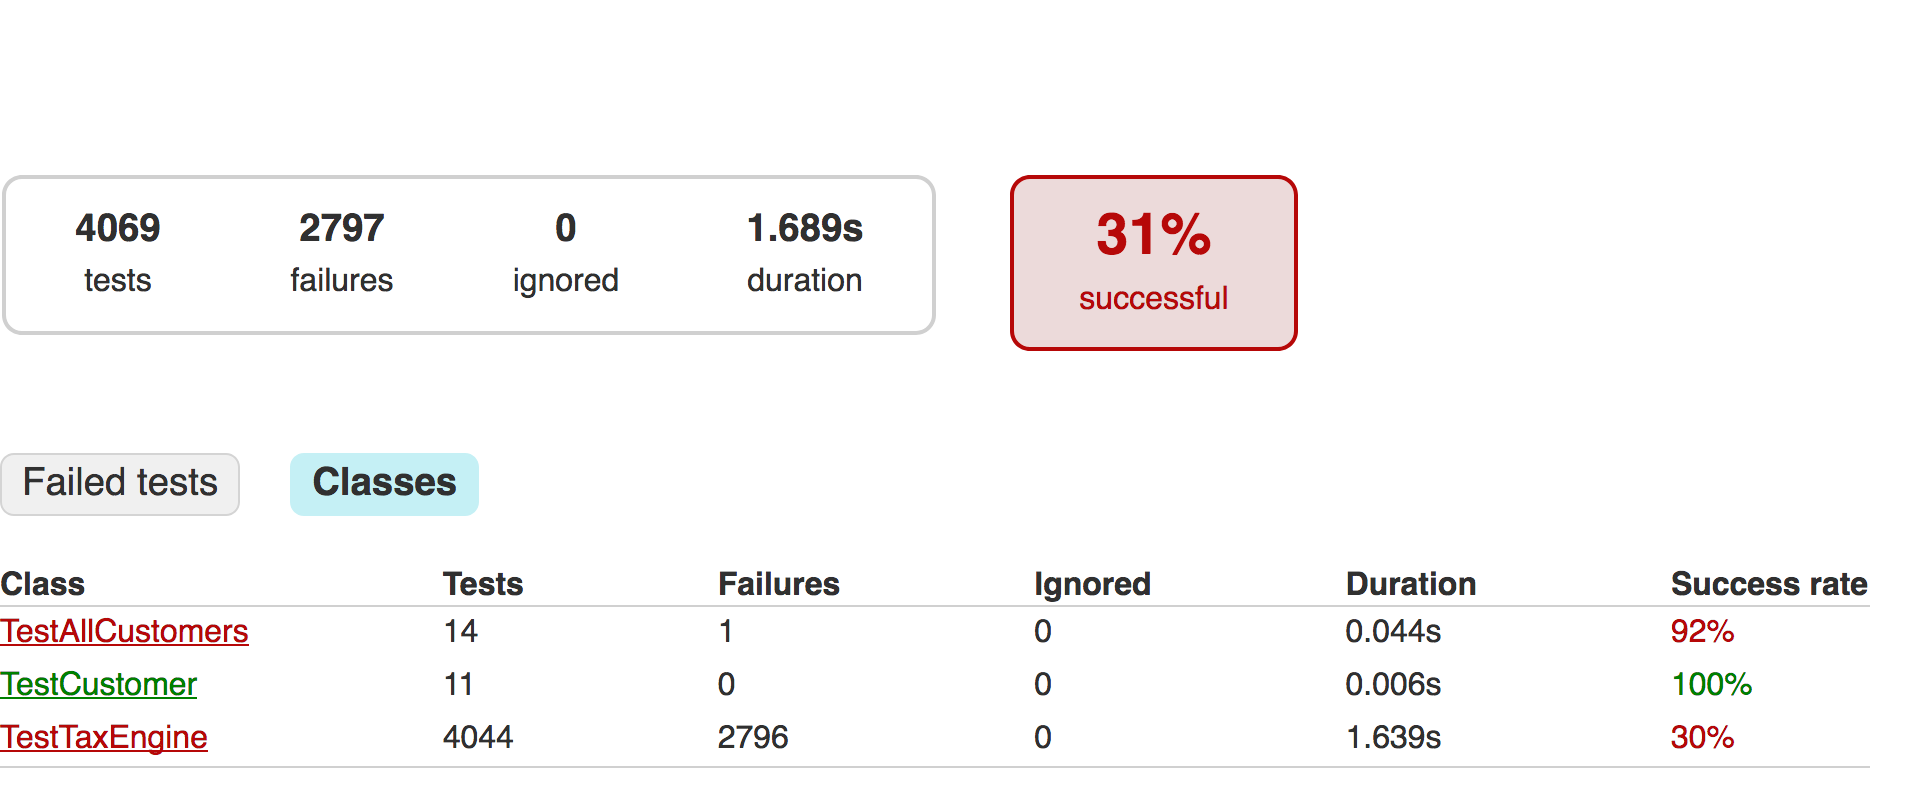
\includegraphics[scale=0.5]{res/unit-test.png}
\caption{JUnit Test Report}    
\end{mdframed}
\end{figure}
% ============================================================================

% ============================================================================
% STYLE CHECKS
\subsection{Style Checking}

% ============================================================================

% ============================================================================
% CONTINOUS INTEGRATION
\subsubsection{Jenkins - Continuous Integration}
Continuous integration is a practice in software development to continuously combine all developers’ changes into the main repository several times per day, and run a set of predefined checks to ensure the changes made do not break existing functionality and pre-set standards. 
\par
Doing so means each developer has a near-latest sane copy of the code before making changes allowing for a reduction in the effort expended in tracking defects between different commits  
\par
In doing continuous integration, code changes pushed to the main repository  trigger the CI system to execute the steps defined in the pipeline.
Such steps may include but are not limited to: building the different executables (main and test applications), running unit test suites, acceptance test suites, static analysers (code quality and style checkers) as well as any other defined gradle, shell or other scripts.  
\par
For this project, we setup several Jenkins pipelines which are triggered upon each commit of the code. There are many ways to trigger builds in Jenkins, one such way is to continuously poll the repository for changes. 
Another is to trigger the build manually using HTTP POST. In our test implementation we have written a script found in (scripts/trigger\_jenkins.sh)to trigger the build manually using curl, a Linux tool. The script is run after every commit made. 
\begin{itemize}
    \item TaxCalc-build
	\item TaxCalc-test-acceptance
	\item TaxCalc-test-unit
\end{itemize}

\begin{figure}[H]
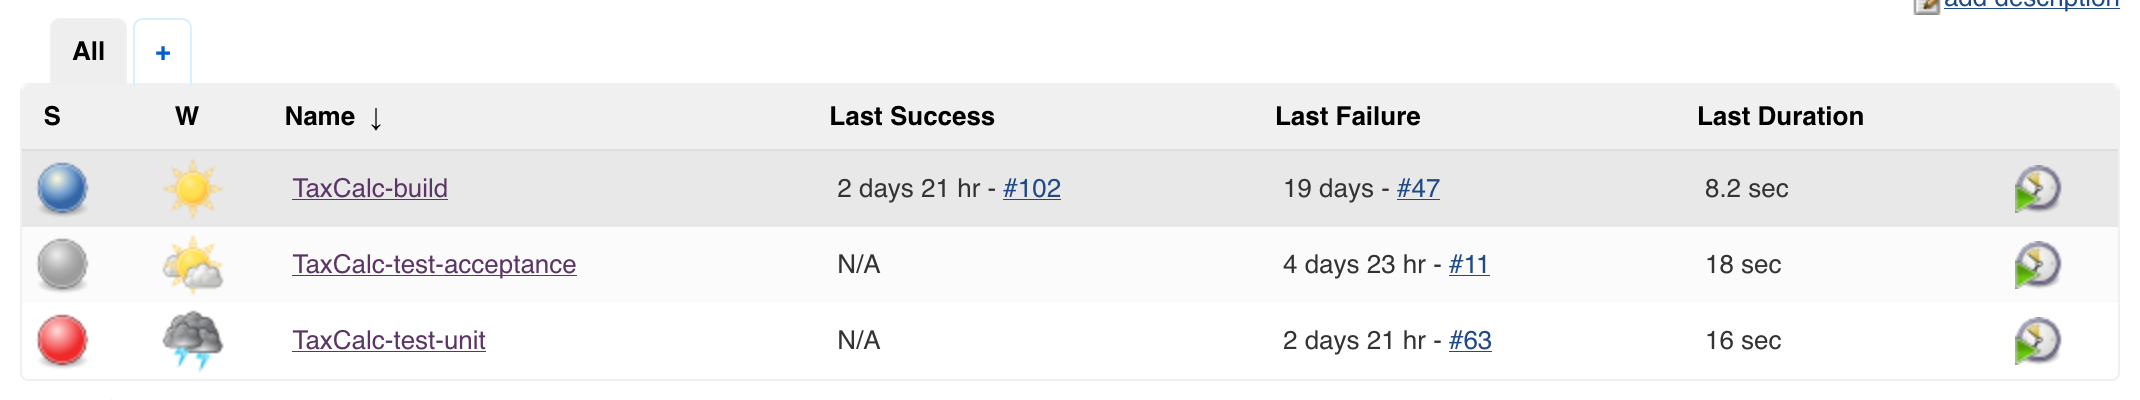
\includegraphics[scale=0.4]{res/jenkins.png}
\label{fig:jenkins-screenshot}
\caption{Screen-shot: Jenkins Project}
\end{figure}
% ============================================================================

% MOVING FORWARD Recommendations
% -------------------------------
% 
% Have a Code Conventions documents 
% BUG TRACKING SOFTWARE 
% Test Driven Development 


% DOCUMENTATION TESTING 
% 
% Documentation
% Developers are required to properly document their in-source code, providing apt descriptions of code functionality, as well as describing how the code contributes to the overall system behaviour. The use of class, sequence and flow diagrams will be encouraged and enforced in certain cases. Doxygen, an open-source documentation generation tool will be used to create web-pages describing code and system behaviour. Doxygen is widely used and easy to learn.
% Recommended tool: Doxygen / JavaDoc


% ============================================================================
% DEFECTS LIST
\subsection{List of defects}

This section outlines the list of found defects in the tables categorised by severity. These defects do not include the requirement defects which have already been in section \ref{sec:defects-and-vaguenesses}. 
\par 

Most "High severity" defects have an associated behavioural test that correctly flags them in our test suite, which greatly helps identify whether future bug fixes do indeed resolve them.

\subsubsection{High severity defects}
\begin{table}[H]
\footnotesize 
\begin{tabularx}{\textwidth}{| c | P | X | X | P |}
% ===================================================================================
\hline % =================================    HEADER  ====================================================
\tblheader{ID} & \tblheader{Component} & \tblheader{Description} & \tblheader{Recommendation} & \tblheader{Test} \\
\hline % ============================================================================

% ===================================================================================
D022 
& TaxEngine 
& First letters in tax code is always ignored.   
& Replace instances of "taxCode.indexOf() > 0" with "taxCode.indexOf() >= 0".
&  Feature8 (Extensive) \\% + Cannot be detected using 'MT1000' and 'TM1000' because the current implementation is faulty due to it only checking lower case characters. If we temporarily remove case sensitivty from the taxAmount() parser code, then we can see that this test fails on the original implementation\\
\hline % ============================================================================
D023 
& TaxEngine 
& Mutual exclusivity between letters in a same tax group is not enforced by the application.
& Use a better regular expression (see CorrectTaxEngine.java).
& Feature 8 Scenario 2 \\
\hline % ============================================================================
D026 
& TaxEngine 
& Tax codes with format similar to '100M100' are not invalidated by the application.
& Use a better regular expression (see CorrectTaxEngine.java). 
& Feature 8 Scenario 3 \\
\hline % ============================================================================

D024 
& TaxEngine 
& Wrongly formatted taxcode yields a zero taxable amount as an error. Zero is a valid taxable amount and does not represent an error. 
& Throw an exception instead.
& Feature 8 (many)\\
\hline % ============================================================================
D001 
& AllCustomers 
& Customer's tax amount is not updated following a salary update (command 'y'). 
& Call taxEngine.taxAmount() in updateCustomerSalary(). 
& Feature 3 Scenario 4 \\
\hline % ============================================================================
D002 
& AllCustomers 
& Customer's tax amount is not updated following a full update (command 'u').
& Call taxEngine.taxAmount() in updateCustomerAll(). 
& Feature 3 Scenario 5\\
\hline % ============================================================================
D009 
& AllCustomers 
& "getCustomer" loops from 0 to intCurrentCustomerIndex inclusive leading to a NullPointerException
& Loop up to intCurrentCustomerIndex - 1 instead.
& JUnit \linebreak {\tiny testGetInexistentCustomer()} \\
\hline % ============================================================================
D008 
& Main
& All previous data is lost following an invalidate user input (Main reinstantiates allCustomers in InterpretCommand()).
% Main creates a new AllCustomers object upon an exception, so if the user inputs something wrong, then an exception is thrown and data about all customers previously is lost 
& Restructure the run() code so that the exception is caught and handled without having to recall interpret command and reinstantiating AllCustomers. 
& Feature 7 Scenario 1 \\
\hline % ============================================================================
D004 
& Main 
& Printing customers requires knowledge of internal array indices.  
& Allow users to print customers using comma-separated list of IDs.
& -\\
\hline % ============================================================================
\end{tabularx}
\caption{High severity functional defects}
\end{table}

% ============================ > SPLIT TABLE

\begin{table}[H]
\footnotesize 
\begin{tabularx}{\textwidth}{| c | P | X | X | P |}
% ===================================================================================
\hline % =================================    HEADER  ====================================================
\tblheader{ID} & \tblheader{Component} & \tblheader{Description} & \tblheader{Recommendation} & \tblheader{Test} \\
\hline % ============================================================================
D036 
& TaxEngine
& Married customer (salary < 27,000) is taxed at 150\% instead of 120\%
& Use HIGH\_MARRIED\_MODIFIER instead of HI\_MARRIED\_MODIFIER
& Feature 8 (a) Scenario 1\\
\hline % ============================================================================
D037
& TaxEngine
& Divorced customer (salary < 24,000) is taxed 118\% instead of 95\%
& Use HIGH\_DIVORCED\_MODIFIER instead of HI\_DIVORCED\_MODIFIER.
& Feature 8 (a) Scenario 2\\
\hline % ============================================================================
D038
& TaxEngine
& Customer with 2 children (salary > 9,900) is taxed ten times more than he should be. 
& Replace TOP\_CHILD2\_MODIFIER = 10.1, with TOP\_CHILD2\_MODIFIER = 1.01.
& Feature 8 (a) Scenario 3\\
\hline % ============================================================================
D039
& TaxEngine
& Customer is student less than 24 y.o (salary < 2,000) is taxed 113\% instead of 107\%. 
& Swap values of HI\_STUDENT1\_MODIFIER and LOW\_STUDENT1\_MODIFIER in Constants.
& Feature 8 (a) Scenario 4\\
\hline % ============================================================================
D040
& TaxEngine
& Customer is student less than 24 y.o (salary < 3,000) is taxed 125\% instead of 113\%
& Use TOP\_STUDENT1\_MODIFIER instead of HIGH\_CHILDm\_MODIFIER. 
& Feature 8 (a) Scenario 5\\
\hline % ============================================================================
D041
& TaxEngine
& Customer is student over 24 y.o (salary < 2,000)
& Swap values of LOW\_STUDENT2\_MODIFIER and HI\_STUDENT2\_MODIFIER in Constants
& Feature 8 (a) Scenario 6\\
\hline % ============================================================================
D042
& TaxEngine
& Customer is student over 24 y.o (salary < 3,000)
& Swap values of LOW\_STUDENT2\_MODIFIER and HI\_STUDENT2\_MODIFIER in Constants
& Feature 8 (a) Scenario 7\\
\hline % ============================================================================
\end{tabularx}
\caption{High severity functional defects (cont'd)}
\end{table}

\subsubsection{Medium severity defects}
\begin{table}[H]
\renewcommand{\thefootnote}{\roman{footnote}} 
\footnotesize 
\begin{minipage}{\textwidth}

\begin{tabularx}{\textwidth}{| c | P | X | X | P |}
% ========================================================================================================
\hline % =================================    HEADER  ====================================================
\tblheader{ID} & \tblheader{Component} & \tblheader{Description} & \tblheader{Recommendation} & \tblheader{Test} \\
\hline % =================================================================================================
D010 
& Main 
& Updating customer outputs 'customer deleted' instead of 'customer updated'.
& Fix the output message to say updated instead of deleted.
& -\\
\hline % =================================================================================================
D015 
& Main 
& List: printed fields for a customer have no reference to what they refer to.
& Provide a header row indicating the field type in order (firstName, lastName, taxCode...).  
& -\\
\hline % =================================================================================================
D006 
& Main
& PrintMenu: Menu does not expose command ’y’.
& Add line in PrintMenu().
& Feature 9 Scenario 1 \\ % Caught in in step And the application should inform the user that the customer as deleted \\
\hline % =================================================================================================
D007 
& Main
& PrintMenu: Last line of Menu is missing a space to properly align vertical line.
& Add one more space after “QUIT PROGRAM” in PrintMenu(). 
& -\\
\hline % =================================================================================================
D003 
& Customer
& Salary is restricted to $2^{31}−1$
& Change salary type in Customer to Long or BigInteger - otherwise expect issues taxing billionaires. 
& -\\
\hline % =================================================================================================
D019 
& TaxEngine 
& The application does not guard against negative salaries. 
& Use regex and throw an exception.
& Feature 8 (Negative Salaries)\\
\hline % =================================================================================================
D025 \footnote{This was assessed as Medium, because the application did not double-tax when there were duplicates. The defect is just that it did not invalidate the tax code.}
& TaxEngine 
& The application does not invalidate the taxcode if there were duplicates of the same letter. 
& Use regex and throw an exception.
& -\\
\hline % =================================================================================================
D013 
& TaxEngine 
& User can see the output from regex matching; this shouldn't be user visible and is confusing.
& Comment out those lines, or use a proper logging library. 
& -\\
\hline % =================================================================================================
\end{tabularx}
\caption{Medium severity functional defects}
\end{minipage}
\end{table}

\subsubsection{Low severity defects}
\begin{table}[H]
\footnotesize 
\begin{tabularx}{\textwidth}{| c | P | X | X | P |}
% ========================================================================================================
\hline % =================================    HEADER  ====================================================
\tblheader{ID} & \tblheader{Component} & \tblheader{Description} & \tblheader{Recommendation} & \tblheader{Test} \\
\hline % =================================================================================================
D011 
& Main 
& Inconsistent word choice and formatting (e.g. changed, modified, updated..). Avoid ".." at the end of output messages.
& Define a consistent output structure and format and enforce it. 
& - \\
\hline % =================================================================================================
D034 
& Main
& No alert when attempting to delete a non-existent entry. 
& Provide an error output when the user attempts this operation. 
& Feature 9 Scenario 2\\
\hline % =================================================================================================
D028 
& Main
& PrintMenu: some functions are displayed in lower case others in upper case.  
& Choose a consistent format. 
& -\\
\hline % =================================================================================================
D029 
& Main
& PrintMenu: FIRST name, SURNAME, TAX CODE, details. All kinds of capitals  
& Choose a consistent format. 
& -\\
\hline % =================================================================================================
D035 
& Main
& addCustomer and updateCustomer differ in the order with which they request input (tax code then salary / salary then tax code) 
& Reorder the readLine()/readInt() methods along with their respective println() statements
& -\\
\hline % =================================================================================================
D030 
& Main 
& If user provides index $first > last$ for range, no error message is output. 
& Provide an error output when the user provides 
& -\\
\hline % =================================================================================================
D031 
& Main 
& First name and last name have no validation whatsoever: they can be empty strings, just numbers and just odd characters. Use some form of validation  
& Regular expressions can be employed to validate input format.  
& -\\
\hline % =================================================================================================
D032 
& Main
& Application unexpectedly prints the menu after 'list', 'add', 'delete' command are done.   
& Consume the new line after reading integers with readInt(). 
& -\\
\hline % =================================================================================================
D033 
& TaxEngine
& "fourth group" message inconsistently with similar messages, starts with a capital letter. This message should not be output in the first place (see D013). 
& Remove this and related debug messages (see D013), or be consistent in formatting. 
& -\\
\hline % =================================================================================================
D014 
& Customer
& Code style: getter/setter methods do not match their member variables (e.g. lastName).
& Example: member name should have setter and getter: setName() and getName().
& -\\
\hline % =================================================================================================
\end{tabularx}
\caption{Low severity functional defects}
\end{table}

% ============================================================================

% ============================================================================
% APPENDIX
\appendix

\setcounter{section}{0}
\pagebreak 
\clearpage
\thispagestyle{empty} % remove page number
\vspace*{9cm}
\begin{center}
{\bf \LARGE Appendix}
\end{center}
\vfill
\pagebreak


\section{Labelled Requirements}
\label{appendix:labelled-requirements}
	\begin{table}[H]
	\small
	\centering
	\begin{tabularx}{\textwidth}{| c | X |}
    \hline %  -----------   Header  ---------------------------------
    \tblheader{Label} & \tblheader{Requirement} \\
    \hline %  -----------   Header  ---------------------------------
    R1 & The application must enable the storage of client’s personal details including: 
    \begin{itemize}[itemsep=\tableitemsep, leftmargin=\tableleftsep]
    \item First Name
    \item Last (family) name
    \item Current salary (as a whole number in GB pounds. No ‘pence’ required)
    \item Tax code 
\end{itemize}
\\
    \hline % ---------------------------------------------------------
    R2 &  The software should issue each customer a numeric identifier which must be unique to that client and never be used by a different client (that is, if a client is deleted from the system then their ID should not be used again but has to ‘die’ with them). \\
	\hline % ---------------------------------------------------------
	R3 & The application should be able to print lists of customer information with users being able to select blocks of customers to be printed based on their unique identifiers. \\
	\hline % ---------------------------------------------------------
	R4 & The application will calculate the tax amount to be paid by each client and display this amount along with the other customer details. The amount of the tax is based on their tax code and their current salary according to the rules below. \\
	\hline % ---------------------------------------------------------
	R5 & The system must include a simple ‘help’ system that lists all commands \\
	\hline % ---------------------------------------------------------
	R6 & The system must not crash if the user enters something that they are not meant to. \\
	\hline % ---------------------------------------------------------
	& The tax rules are as follows:\\
	\hline % ---------------------------------------------------------
	R7.1 & Tax amount can be calculated from a person’s tax code and their current salary. \\
	\hline % ---------------------------------------------------------
	R7.2 & A tax code has a numerical part and an alphabetic part. For compatibility with legacy
	tax code policy, the numeric and alphabetic portion of the tax code may be presented in either order. Thus, for clarity, both of the following tax codes are valid:
	\begin{itemize}[itemsep=\tableitemsep, leftmargin=\tableleftsep]
	\item 1080MT
	\item SF980
\end{itemize}
	\\
	\hline % ---------------------------------------------------------
	R7.3 & The numeric part of the tax codes represents a ‘base’ tax amount that is then modified by the alphabetic portion of the tax code and depending on the person’s current salary. \\
	\hline %  -----------   Header  ---------------------------------
    R7.4 & The alphabetic portion of the code may consist of multiple letters drawn from the following set, with their corresponding meanings: 
    \begin{itemize}[itemsep=\tableitemsep, leftmargin=\tableleftsep]
    \item ‘M’ : Married
    \item ‘S’ : Single
    \item ‘D’ : Divorced
    \item ‘C’ : Has a single child
    \item ‘E’ : Has two children
    \item ‘F’ : Has multiple (more than two) children 
    \item ‘T’ : Full-time student below the age of 24 
    \item ‘U’ : Full time student 24 years and older
\end{itemize}
	\\
	\hline % ---------------------------------------------------------
	\end{tabularx}
	\end{table}

	% ----------------------------> 
	% Split the table to two pages 
	% ----------------------------> 

	\begin{table}[H]
	\small
	\centering
	\begin{tabularx}{\textwidth}{| c | X |}
    \hline %  -----------   Header  ---------------------------------
    \tblheader{Label} & \tblheader{Requirement} \\
	\hline % ---------------------------------------------------------
	R7.5 & Calculation of tax for Married people: one of the following four bands will apply:
	\begin{itemize}[itemsep=\tableitemsep, leftmargin=\tableleftsep]
		\item Married people with a current salary of less than £5000 will pay a tax rate of
		70\% of their base tax amount.
		\item Married people with a current salary less than £12,000 will pay a tax rate of
		90\% of their base tax amount.
		\item Married people with a current salary less than £27,000 will pay a tax rate of
		120\% of their base tax amount
		\item Married people with a current salary above than £27,000 will pay a tax rate
		of 130\% of their base tax amount
	\end{itemize}
	\\
	\hline % ---------------------------------------------------------
	R7.6 & Calculation of tax for Single people: one of the following four bands will apply:
	\begin{itemize}[itemsep=\tableitemsep, leftmargin=\tableleftsep]
		\item Single people with a current salary of less than £6500 will pay a tax rate of 75\% of their base tax amount.
		\item Single people with a current salary less than £11,000 will pay a tax rate of 95\% of their base tax amount.
		\item Single people with a current salary above £22,000 will pay a tax rate of 125\% of their base tax amount
		\item Single people with a current salary above than £22,000 will pay a tax rate of 132\% of their base tax amount
	\end{itemize}
	\\
	\hline % ---------------------------------------------------------
	R7.7 & Calculation of tax for divorced people: one of the following four bands will apply:
	\begin{itemize}[itemsep=\tableitemsep, leftmargin=\tableleftsep]
		\item Divorced people with a current salary of less than £7200 will pay a tax rate
		of 60\% of their base tax amount.
		\item Divorced people with a current salary less than £13,000 will pay a tax rate of
		80\% of their base tax amount.
		\item Divorced people with a current salary above £24,000 will pay a tax rate of
		95\% of their base tax amount
		\item Divorced people with a current salary above than £24,000 will pay a tax rate
		of 110\% of their base tax amount
	\end{itemize}
	\\
	\hline % ---------------------------------------------------------
	R7.8 & Calculation of tax for people with a single child. One of the following three bands will apply:
	\begin{itemize}[itemsep=\tableitemsep, leftmargin=\tableleftsep]
		\item People with a single child and a current salary of less than £8000 will pay a tax rate of 80\% of their base tax amount after taking into consideration any
		adjustments due to their marital status
		\item People with a single child and a current salary of less than £10400 will pay a
		tax rate of 85\% of their base tax amount after taking into consideration any
		adjustments due to their marital status
		\item People with a single child and a current salary greater than £10400 will pay a
		tax rate of 95\% of their base tax amount after taking into consideration any adjustments due to their marital status
	\end{itemize}
	\\
	\hline % ---------------------------------------------------------
\end{tabularx}
\end{table}
	% ----------------------------> 
	% Split the table to two pages 
	% ----------------------------> 

\begin{table}[H]
\small
\centering
\begin{tabularx}{\textwidth}{| c | X |}
	\hline % ---------------------------------------------------------
	R7.9 & Calculation of tax for people with two children. One of the following three bands will apply:
	\begin{itemize}[itemsep=\tableitemsep, leftmargin=\tableleftsep]
		\item People with a two children and a current salary of less than £7400 will pay a tax rate of 90\% of their base tax amount after taking into consideration any adjustments due to their marital status
		\item People with a two children and a current salary of less than £9900 will pay a tax rate of 95\% of their base tax amount after taking into consideration any adjustments due to their marital status
		\item People with a two children and a current salary greater than £9900 will pay a tax rate of 101\% of their base tax amount after taking into consideration any adjustments due to their marital status
	\end{itemize}
	\\
	\hline % ---------------------------------------------------------
	R7.10 & Calculation of tax for people with more than two children. One of the following three bands will apply:
	\begin{itemize}[itemsep=\tableitemsep, leftmargin=\tableleftsep]
		\item People with more than two children and a current salary of less than £7000 will pay a tax rate of 120\% of their base tax amount after taking into consideration any adjustments due to their marital status
		\item People with more than two children and a current salary of less than £9000 will pay a tax rate of 125\% of their base tax amount after taking into consideration any adjustments due to their marital status
		\item People with more two children and a current salary greater than £9000 will pay a tax rate of 130\% of their base tax amount after taking into consideration any adjustments due to their marital status
	\end{itemize}
	\\
	\hline % ---------------------------------------------------------
	R7.11 & Calculation for people who are in full time education who are below that age of 24 : One of the following three bands will apply (adjustments to be made after taking into account marital status and number of children):
	\begin{itemize}[itemsep=\tableitemsep, leftmargin=\tableleftsep]
		\item People in full-time education below the age of 24 and have a current salary less than £2000 will pay a tax rate of 107\%
		\item People in full-time education below the age of 24 and have a current salary less than £3000 will pay a tax rate of 113\%
		\item People in full-time education below the age of 24 and have a current salary more than £3000 will pay a tax rate of 123\%
	\end{itemize}
	\\
	\hline % ---------------------------------------------------------
	R7.12 & Calculation for people who are in full time education who are 24 years of age and above : One of the following three bands will apply (adjustments to be made after taking into account marital status and number of children):
	\begin{itemize}[itemsep=\tableitemsep, leftmargin=\tableleftsep]
	\item People in full-time education, who are 24 and above and have a current salary less than £2000 will pay a tax rate of 109\%
	\item People in full-time education, who are 24 and above and have a current salary less than £3000 will pay a tax rate of 115\%
	\item People in full-time education , who are 24 and above and have a current salary more than £3000 will pay a tax rate of 125\%
	\end{itemize}
	\\
	\hline % ---------------------------------------------------------
\end{tabularx}
\end{table}

% ============================================================================

% ============================================================================
% END DOCUMENT
\end{document}
% ============================================================================

% ============================================================================
% CHECKS
% ============================================================================

% [  ] Check spelling
% [  ] Check with "grammarly"

% =============================================================================
% DRAFT
% =============================================================================